\section{Problems and Solutions}
\markright{Problems and Solutions}

\subsection{Problem 1: Hello World}
This program demonstrates the minimal structure of a C++ application and how to print a line of text to the standard output.

\subsubsection{Code}
\begin{lstlisting}[language=C++, caption={Hello World Program}, numbers=left]
#include <iostream>

int main() {
    std::cout << "Hello World" << std::endl;
    return 0;
}
\end{lstlisting}

\subsubsection{Output}
\begin{figure}[H]
  \centering
  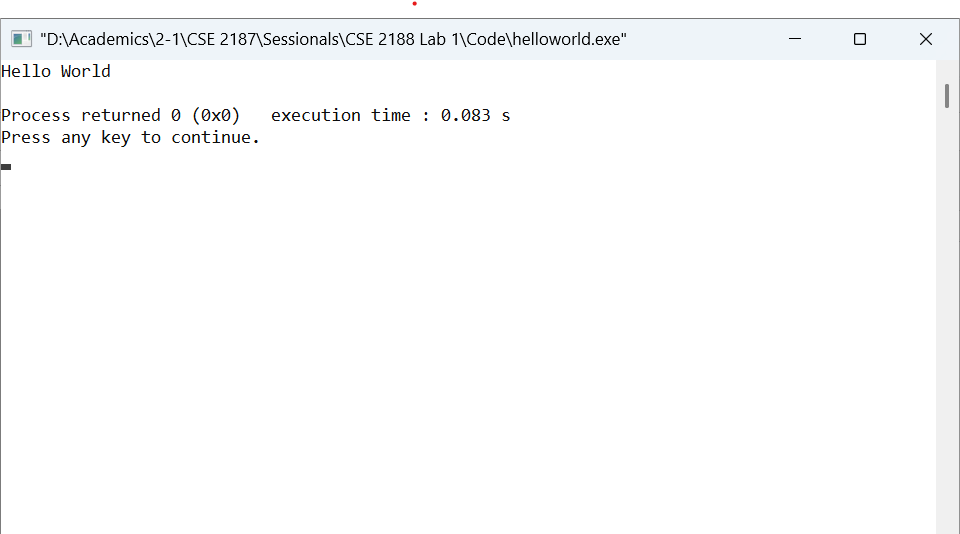
\includegraphics[width=0.8\textwidth]{lab-01/assets/output1.png}
  \caption{Output of the Hello World Program.}
\end{figure}

\subsection{Problem 2: User Interaction}
This program shows how to declare strings, prompt the user for input, read the input, and then display a formatted message using the information provided by the user.

\subsubsection{Code}
\begin{lstlisting}[language=C++, caption={User Interaction Program}, numbers=left]
#include <iostream>

int main() {
    char name[100], hobby[100], home[100];

    std::cout << "What's your name? ";
    std::cin >> name;

    std::cout << "Where are you from? ";
    std::cin >> home;

    std::cout << "What's your favorite hobby? ";
    std::cin >> hobby;

    std::cout << "\nHi! " << name << " from " << home << "! Enjoy " << hobby << "!" << std::endl;
    return 0;
}
\end{lstlisting}

\subsubsection{Output}
\begin{figure}[H]
  \centering
  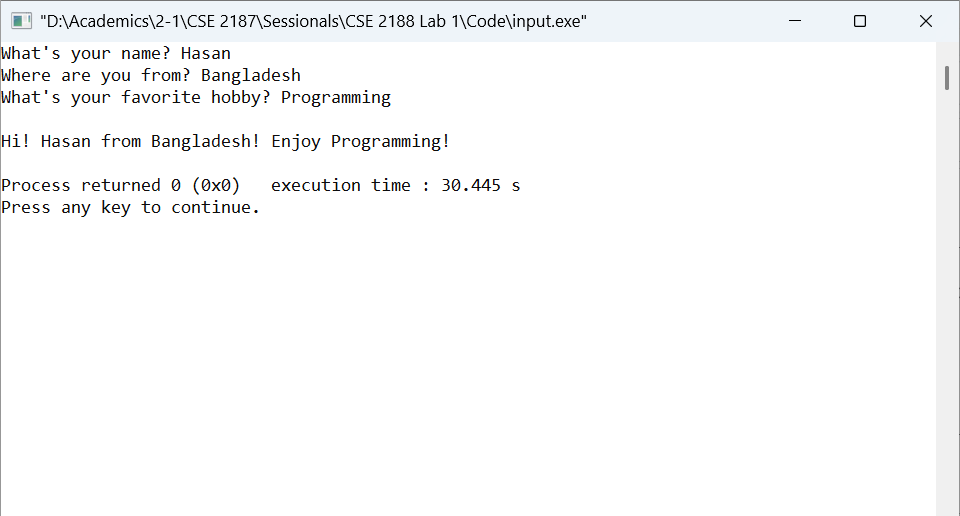
\includegraphics[width=0.8\textwidth]{lab-01/assets/output2.png}
  \caption{Output of the User Interaction Program.}
\end{figure}
